\chapter{Ferrofluids}

\section{Introduction}

\par A \textbf{ferrofluid} is a colloidial suspension composed of small (3-15 nm) solid, single-domain, magnetic particles coated with a molecular layer of a dispersant and suspended in a liquid carrier(Fig. !!). Thermal agitation keeps the particles suspended(under sufficient stability conditions) because of the Brownian motion and the coatings prevents the particles from sticking to each other.

\begin{figure}[ht]
\centering
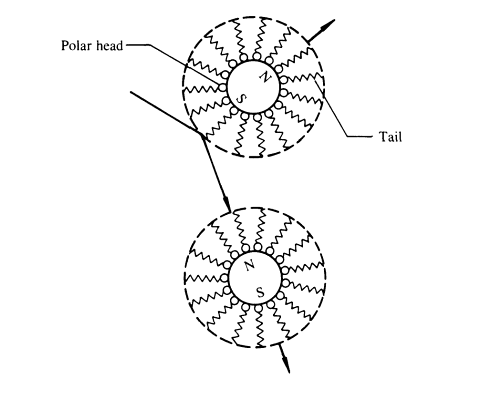
\includegraphics[width=90mm]{img/ferrofluid_schema.png}
\caption{Coated magnetic particles in ferrofluid. Taken from [RW]}
\end{figure}


\par The magnetic ferrofluids of the type in general use today are an outgrowth of discoveries made in the early 1960s.  \par Because the colloidial ferrofluid is not found in the nature is must be synthetized. Methods called \textit{size reduction} and \textit{chemical precipitation} are used. Details of both methods can be found in [RW].

\par Very important property of ferrofluid is its stability. It ensures the investigator of well-defined material for scientific studies and also fluid applications. We mean 
\begin{itemize}
\item \textit{stability in a magnetic field gradient},
\item \textit{stability against settling in a gravitational field},
\item \textit{stability against magnetic agglomeration} and
\item \textit{neccesity to guard against the van der Waals attractive force.}
\end{itemize}

\par To derive the physicochemical stability dimensionless analysis can be used introducing various energy terms:

\begin{itemize}
\item \textit{thermal energy} $kT$,
\item \textit{magnetic energy} $\mu_0 M H V$ and
\item \textit{gravitational energy} $\Delta \rho V g L$,
\end{itemize}

where $k$ is Boltzmann's constant, $T$ the absolute temperature in degrees Kelvin, $\mu_0$ is the permeability of free space, $V$ volume of a sperical particle, $L$ the elevation in gravitational field, $\Delta \rho$ difference in fluid carrier and ferromagnetic particles densities and $M, H$ magnetization and magnetic field intensity.

\par Such stability analysis leads to inequalities for  the particle diameter, for instance, for the magnetite($\mathrm{Fe}_3 \mathrm{O}_4$)  particles at the room temperature stability against magnetic agglomeration requires diameter $d \leq 7.8 ~ \si{\nano\metre}$ [RW]. 

\section{Ferrohydrodynamics}

\par The term \textbf{ferrohydrodynamics} (FHD) was first introduced by \textbf{Ronald E. Rosensweig}. Development of FHD in early to mid- 1960s was motivated by engineering task of converting heat to work with no mechanical parts. 

\say{\textit{Ferrohydrodynamics is an interdisciplinary topic having inherent interest of a physical and mathematical nature with applications in tribology, separations science, instrumentation, information display, printing, medicine, and other areas}} R.E.Rosensweig. 

\par In the begining of this chapter we would like to emphasize the differences between various studies of fluid--field interactions: 

\begin{enumerate}
\item \emph{electrohydrodynamics} (EHD) deals with the influence of the electric field on a fluid motion,
\item \emph{magnetohydrodynamics} (MHD) is the study of the interaction between magnetic field and fluid conductors of electricity,
\item \emph{ferrohydrodynamics} (FHD) deals with the mechanics of fluid motion influenced by forces of magnetic polarization.
\end{enumerate}

\par This work is mainly concerned with ferrohydrodynamics, because ferrofluids are non--conducting therefore there is zero Lorentz force acting as body force(in contrast with MHD). The body force in FHD is due to \emph{polarization force} which requires material magnetization in presence of magnetic field gradients or discontinuities. 

\subsection{Magnetic stress tensor}

\par As we have mentioned above, understanding the differences between several fluid--field interactions play important role in a development of a physical model for the flow of a ferrofluid. 

The only body force acting from the outside in hydrodynamics is gravitational. In electrohydrodynamics electrically charged particles are affected with electrical forces while in magnetohydrodynamics conductive fluid is subject to the Lorentz body force.

\par The derivation of the \emph{magnetic stress tensor} with respect to the thermodynamic background and conservation of energy leads to [RW]

\begin{equation}
\mb{T}_m' = - \left[ p(\rho, T) + \int_0^H \mu_0 \left( \frac{\partial(\nu M)}{\partial \nu} \right)_{H, T} \mathrm{d}H + \frac{1}{2} \mu_0 H^2  \right] \mb I + \mb B \otimes \mb H,
\label{eq:magnetic_stress_tensor}
\end{equation}

where notation from [RW] is adopted so $\mb B \otimes \mb H = B_i H_j$ represents dyadic product, $p$ is thermodynamics pressure, $\rho$ the density, $T$ thermodynamic pressure, $H, M$ associated norm of the magentic field intensity and magnetization respectively, $\mb H, \mb M$, $\mu_0$ permeability of free space, $\nu = \rho^{-1}$ the specific volume, $\mb I$ the identity tensor and $\mb B$ magnetic field induction. 

Note, that the \emph{tensor is symmetric}, because $\mb B \otimes \mb H = \mb H \otimes \mb B$ follows from $\mb B = \mu \mb H$ and $\mb I = \mb I^{\mathrm{T}}$. This result is obtained including nonlinear effects, i.e. nonlinear magnetization of the ferrofluid. In this work a linearly magnetizable ferrofluid is assumed, so the corresponding simplification will be given in the following section.

\subsection{Classification of ``pressures'' in ferrofluid}

In the expression for the magnetic stress tensor, thermodynamic pressure $p = p(\rho, T)$ appeared naturally as a result of the derivation. In order to emphasize the magnetic aspect of the result we define a new tensor $\mb T_m$ such that

$$ \mb T_m := \mb T'_m + p(\rho, T)\mb I $$

so we separated thermodynamic pressure present also in non--polar fluid. The new tensor is

\begin{equation}
\mb T_m = - \left[ \int_0^H \mu_0 \left( \frac{\partial(\nu M)}{\partial \nu} \right)_{H, T} \mathrm{d}H + \frac{1}{2} \mu_0 H^2  \right] \mb I + \mb B \otimes \mb H,
\label{eq:magnetic_stress_tensor_new}
\end{equation}

and the \emph{magnetic force per unit volume} corresponding to a magnetic stress tensor $\mb T_m$ is

\begin{equation}
\mb f_m = \mb \nabla \cdot \mb T_m. 
\label{eq:magnetic_force}
\end{equation}

Assuming few vector identities, Maxwell's equation $\nabla \cdot \mb B = 0$ (non--existence of magnetic monopoles), current--free magnetostatic Ampere's law $\nabla \times \mb H = 0$ and with use of $B = \mu_0(M + H)$ one arrives at 

\begin{equation}
\mb f_m = - \nabla \left[  \mu_0 \int_0^H \left( \frac{\partial(\nu M)}{\partial \nu} \right)_{H, T} \mathrm{d}H   \right] + \mu_0 M \nabla H.
\label{eq:magentic_force_simplified}
\end{equation}

There is an arbitrariness in grouping of magnetic terms in (\ref{eq:magentic_force_simplified}) that has led to some confusion in the literature. Here, we follow the classification introduced in [RW].

Applying the partial derivative in the term $\frac{\partial(\nu M)}{\partial \nu}$ and with use of the identity
$$ \nabla \int_0^H M \mathrm{d}H = M \nabla H + \int_0^H \nabla M \mathrm{d}H $$ we finally have the expression for the magnetic force per unit volume

\begin{equation}
\mb f_m = - \nabla \left[ \mu_0 \int_0^H \nu \left( \frac{\partial M}{\partial \nu} \right)_{H, T} \mathrm{d}H \right] - \mu_0 \int_0^H \nabla M \mathrm{d}H.
\label{eq:magnetic_force_final}
\end{equation}

In the sense of the equation $\mb f = \nabla p$ some pressure--like terms in (\ref{eq:magnetic_force_final}) are identified.

The \textbf{magnetostrictive pressure}

\begin{equation}
p_s := \mu_0 \int_0^H \nu \left( \frac{\partial M} {\partial \nu} \right)_{H,T} \mathrm{d}H
\label{eq:magnetostrictive_pressure}
\end{equation}

and the \textbf{fluid-magnetic pressure}

\begin{equation}
p_m := \mu_0 \int_0^H M \mathrm{d}H.
\label{eq:fluid_magnetic_pressure}
\end{equation}

Applying definitions (\ref{eq:magnetostrictive_pressure}) and (\ref{eq:fluid_magnetic_pressure}) expression for the magnetic stress tensor yelds

$$ \mb T_m = -(p_s + p_m + \frac{1}{2} \mu_0 H^2 ) \mb I + \mu \mb H \otimes \mb H. $$

\subsection{Magnetic force density reduced form}

It could be shown due to \emph{Korteweg and Helmholtz} that for \emph{linearly magnetizable media} magnetic force density reduces to

$$ \mb f_m = \nabla \left[ \frac{H^2}{2} \rho \left( \frac{\partial \mu }{\partial \rho} \right)_{T} \right] - \frac{H^2}{2} \nabla \mu. $$

In this work, \textbf{incompressible linearly magnetizable ferrofluid with magnetization constant within ferrofluid domain} is assumed, therefore it is evident from the Korteweg--Helmholtz expression for the magnetic force that this force vanishes everywhere except for the phase interfaces, where non--zero jump in the permeability is present. 

\subsection{Equation of motion for a ferrofluid}

Very important part of ferrohydrodynamics is devoted to the formulation and study of equation of motion for a ferrofluid. A momentum equation was first proposed by Neuringer and Rosensweig (1964) [NRW]. In order to satisfy the continuum mechanics assumptions, it is assumed, that the dynamic equilibrium holds for and ``infinitesimal element'' which is large enough to contain a large number of colloidial magnetic particles comparing to the dimensions of the flow field.

The Newton's law for such ``infinitesimal'' element yelds

\begin{equation}
\rho \left( \partial_t \mb u + \left(\mb u \cdot \nabla\right) \mb u   \right) = \underset{\text{Pressure force}} {\mb f_p} + \underset{\text{Viscous force}}{\mb f_v} + \underset{\text{Gravity force}}{\mb f_g} + \underset{\text{Magnetic force}}{ \mb f_m } 
\label{eq:newton_ferrofluid}
\end{equation}

The equation (\ref{eq:newton_ferrofluid}) with the magnetic force density expression (\ref{eq:magnetic_force_final}) simply unfolds the effect of a magnetic field on a ferrofluid, but more formal and rigorous problem definition with appropriate simplyfications is given in the form of the \emph{Navier-Stokes equations} in the chapter 4.
 
